% !TEX root = ../main.tex
\documentclass[../main.tex]{subfiles}

\begin{document}
\section{Anhang}
\appendix
\renewcommand{\thesubsection}{\Alph{subsection}}
\subsection{Messaufbauten}

\subsubsection{Gleichstromverstärkung}

\begin{figure}[h]
    \centering
    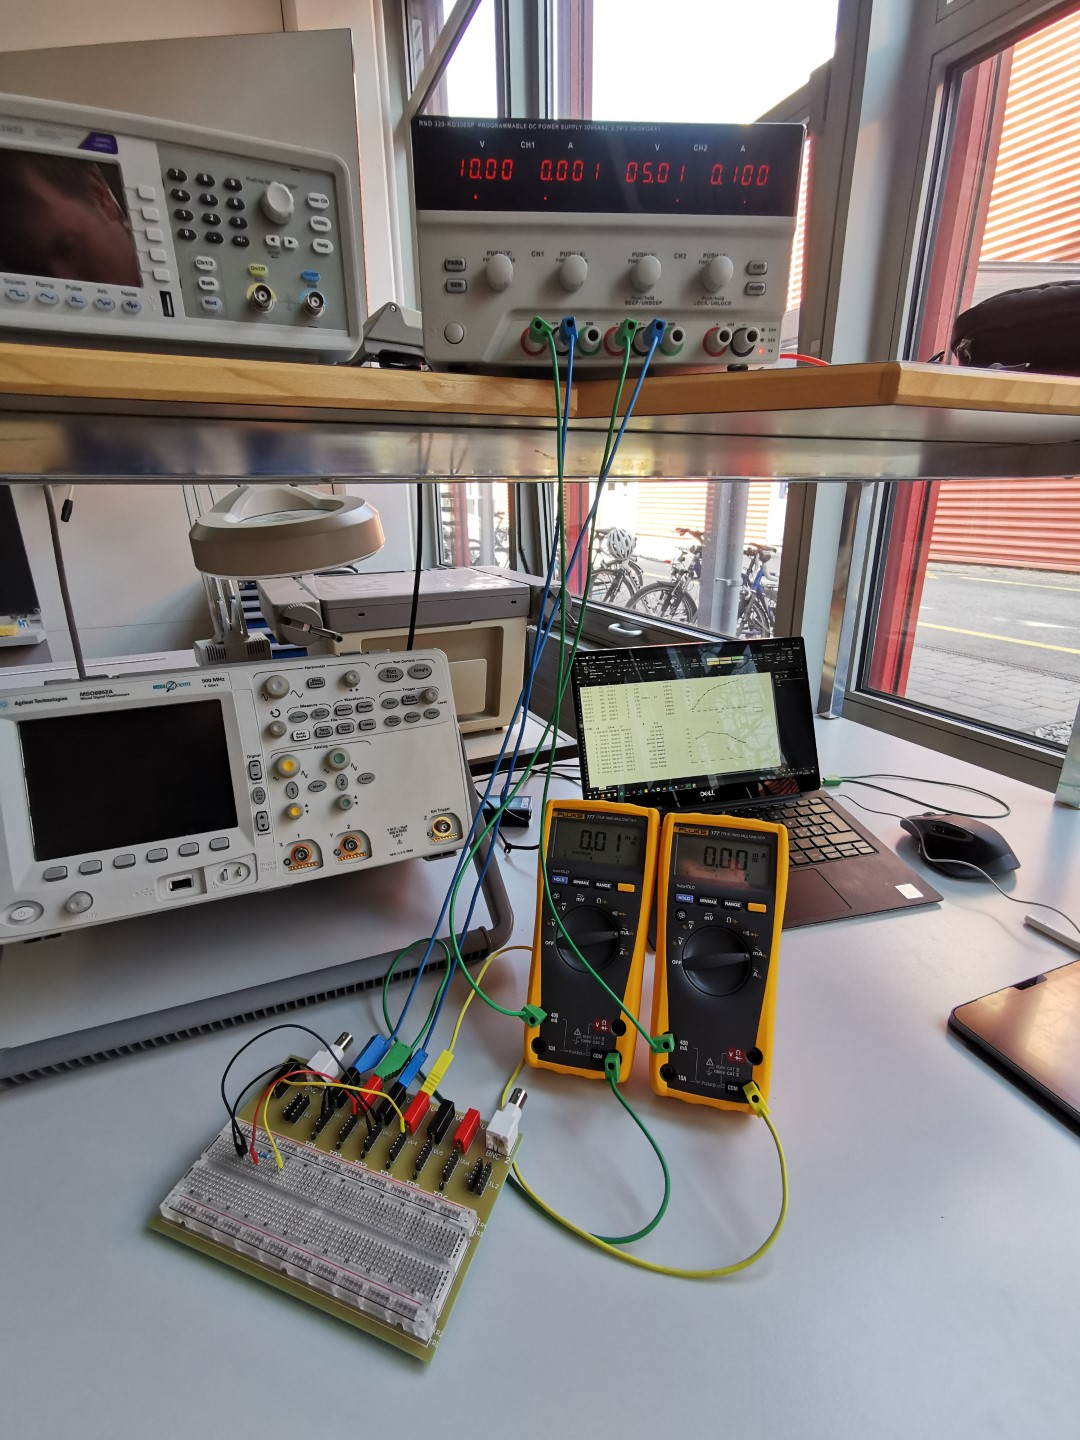
\includegraphics[scale=0.075]{assets/task1_DC_amplification/task1.jpg}
    \caption{Messungsaufbau für die Gleichstromverstärkung-Messung}
    \label{fig:setup_task1}
\end{figure}
\newpage
\subsubsection{Spannungsstabilisierung}

\begin{figure}[h]
    \centering
    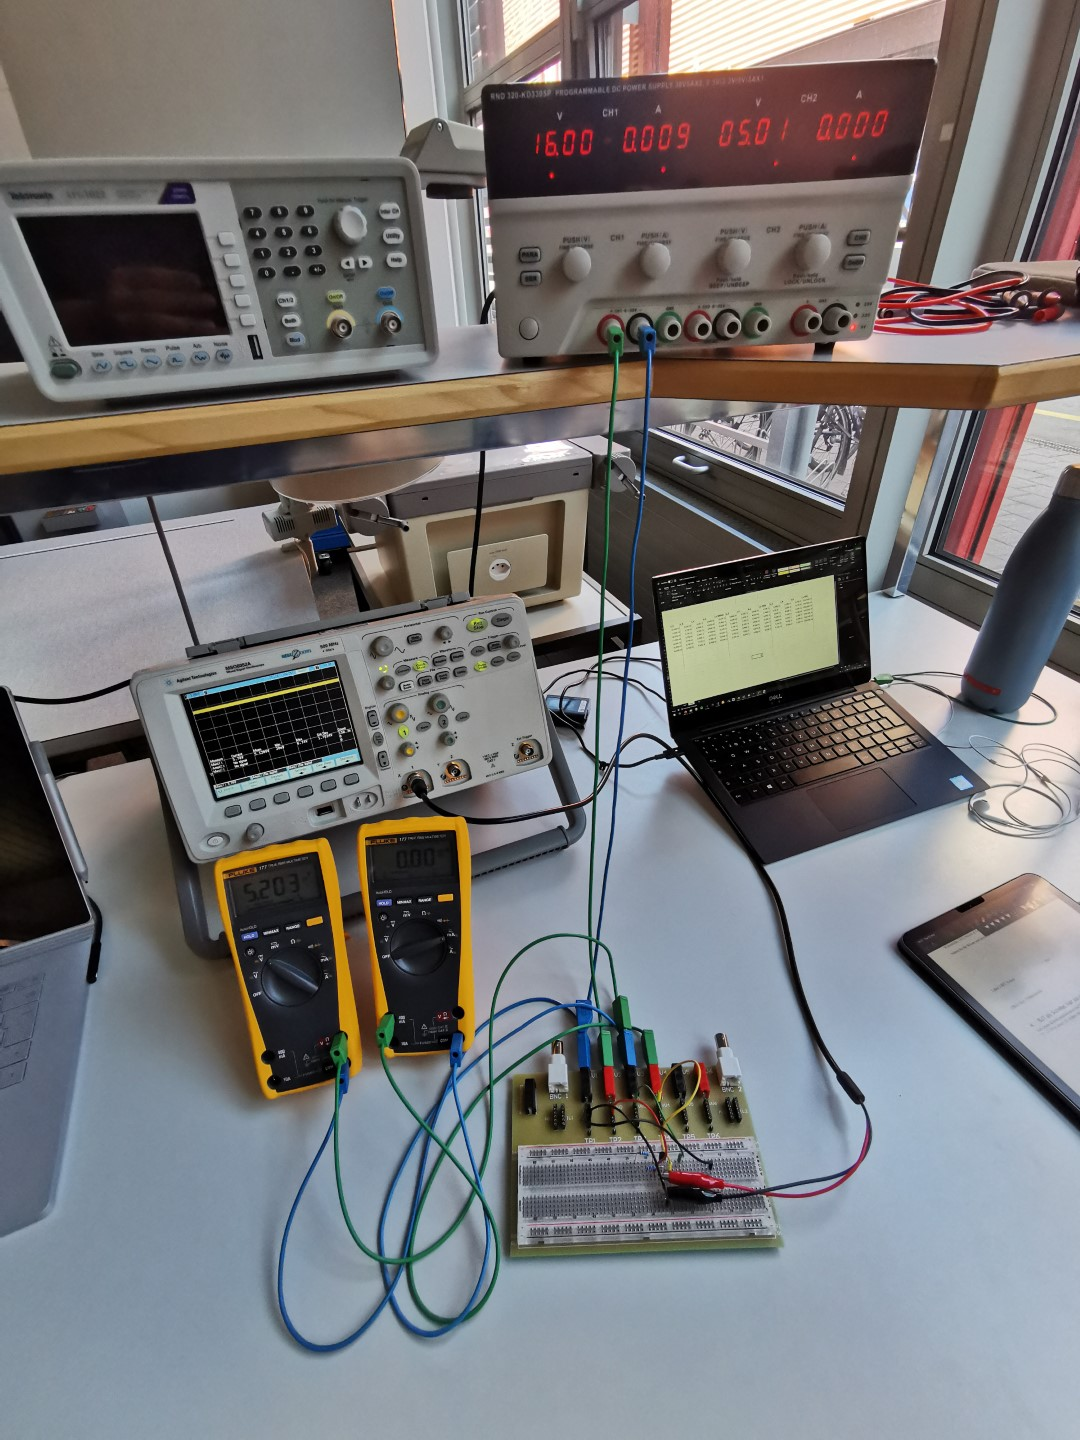
\includegraphics[scale=0.075]{assets/task2_voltage_stable/task2.jpg}
    \caption{Messungsaufbau für die Spannungsstabilisierung-Messung}
    \label{fig:setup_task2_1}
\end{figure}
\newpage
\subsubsection{BJT als Schalter}

\begin{figure}[h]
    \centering
    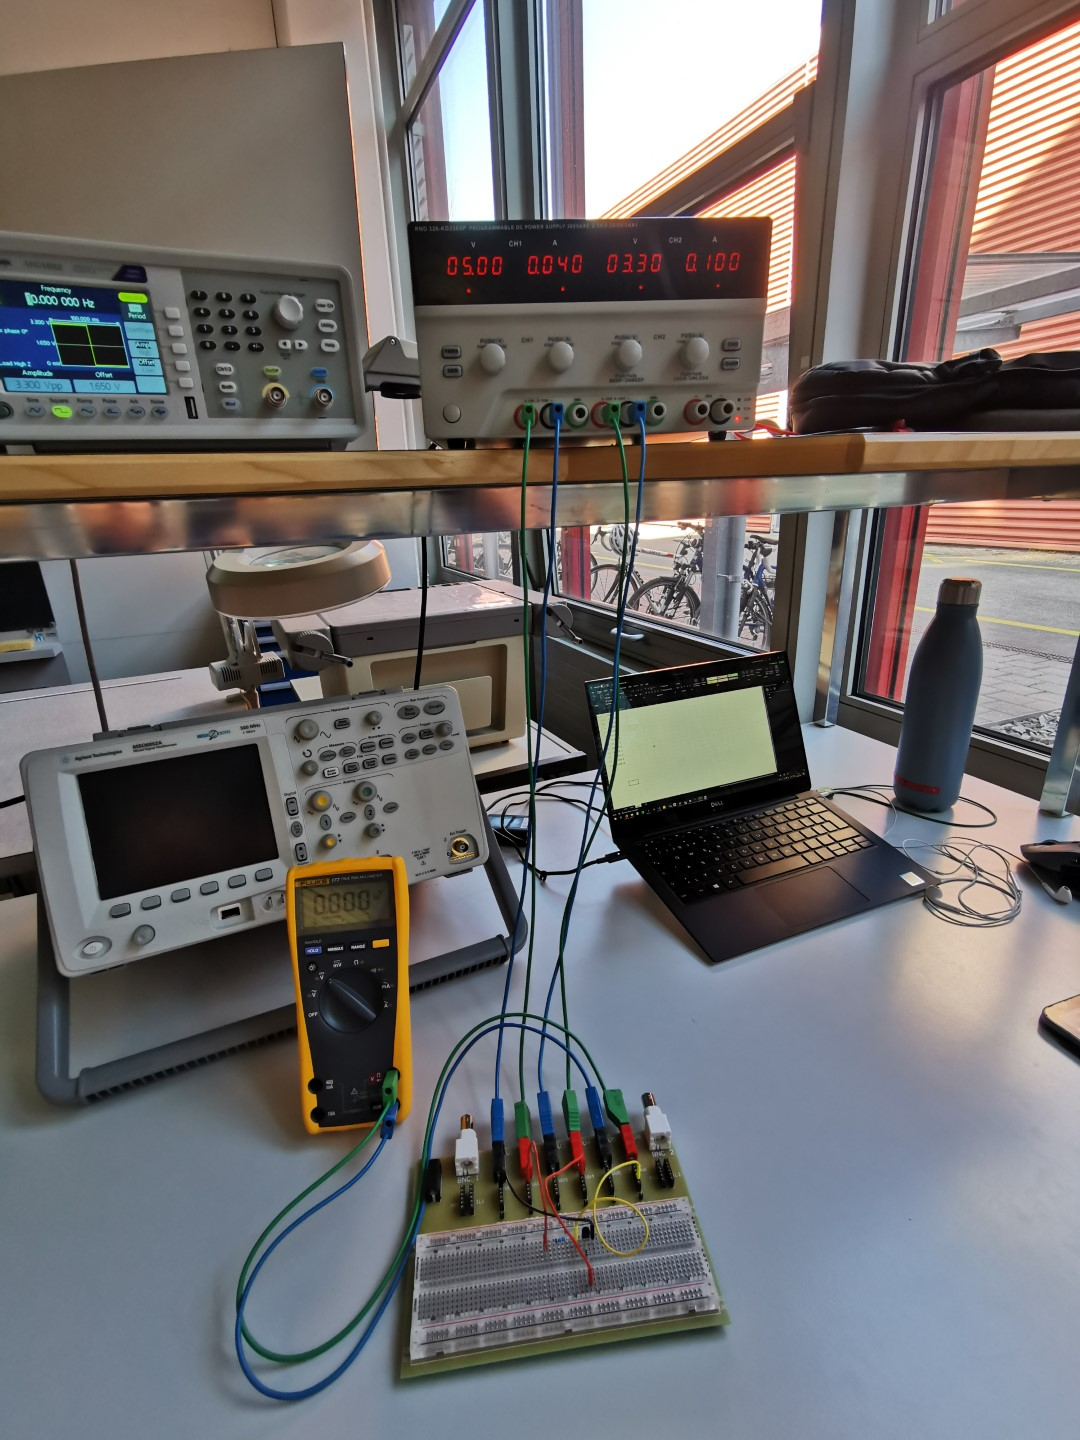
\includegraphics[scale=0.075]{assets/task3_square/task3_2.jpg}
    \caption{Messungsaufbau für die \textit{level shifter}-Messung (DC-Teil der Messung)}
    \label{fig:setup_task3_2}
\end{figure}

\begin{figure}[h]
    \centering
    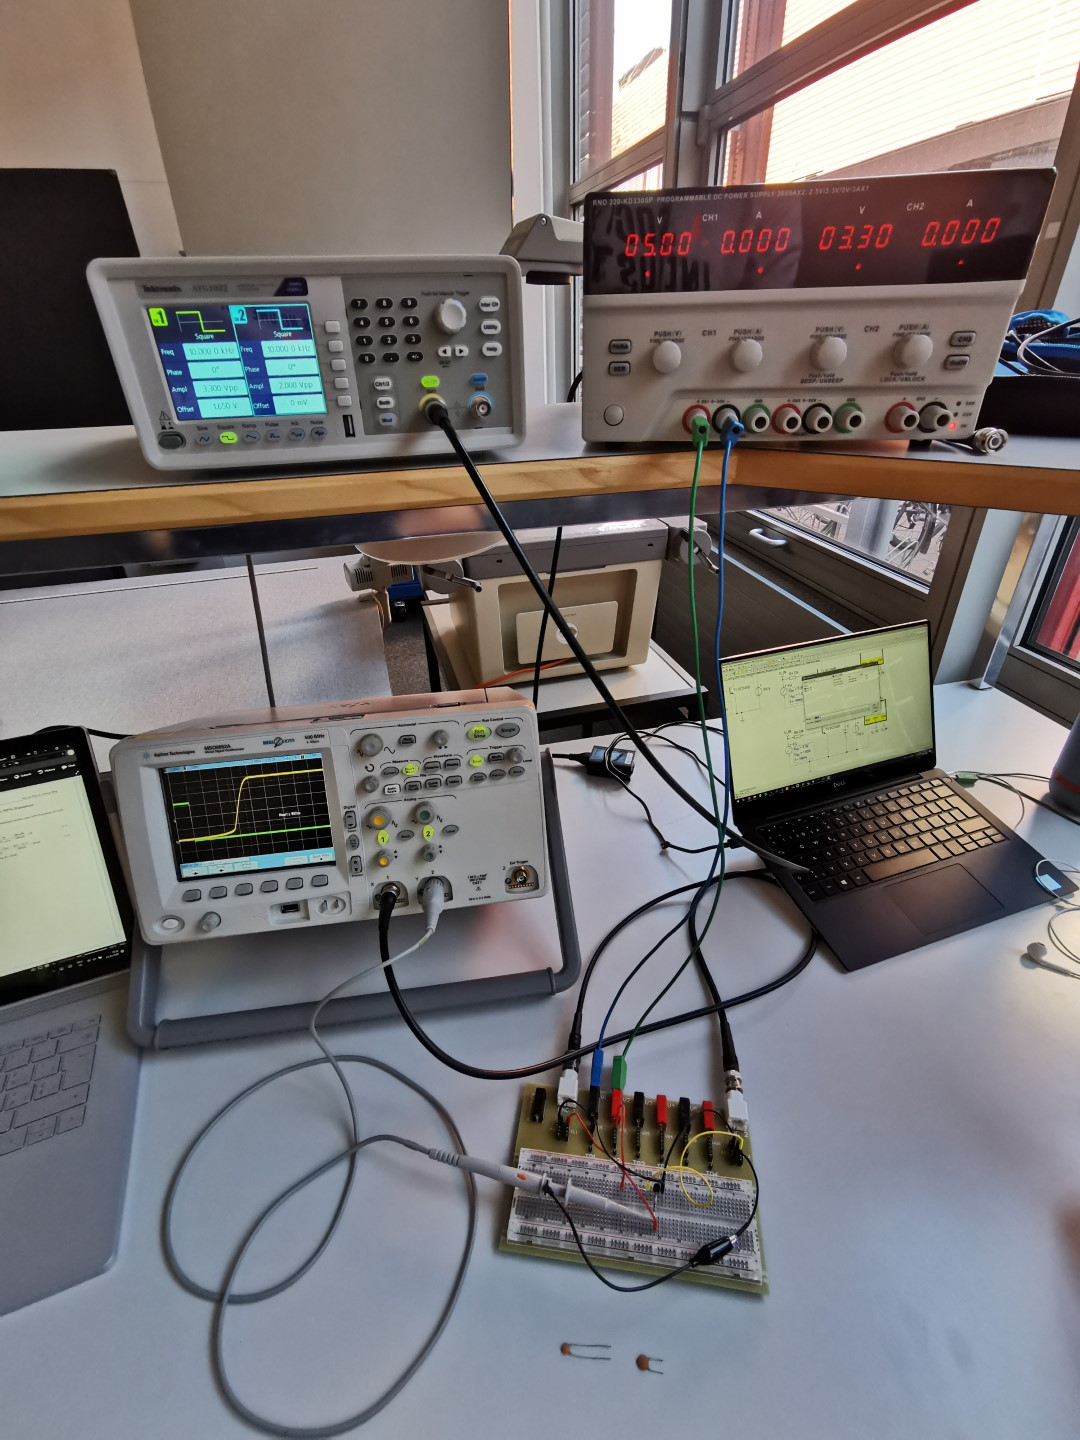
\includegraphics[scale=0.075]{assets/task3_square/task3_1.jpg}
    \caption{Messungsaufbau für die \textit{level shifter}-Messung (AC-Teil der Messung)}
    \label{fig:setup_task3_1}
\end{figure}

\end{document}
